\documentclass{beamer}

\mode<presentation> {

% The Beamer class comes with a number of default slide themes
% which change the colors and layouts of slides. Below this is a list
% of all the themes, uncomment each in turn to see what they look like.

%\usetheme{default}
%\usetheme{AnnArbor}
%\usetheme{Antibes}
%\usetheme{Bergen}
%\usetheme{Berkeley}
%\usetheme{Berlin}
%\usetheme{Boadilla}
%\usetheme{CambridgeUS}
%\usetheme{Copenhagen}
%\usetheme{Darmstadt}
%\usetheme{Dresden}
%\usetheme{Frankfurt}
%\usetheme{Goettingen}
%\usetheme{Hannover}
%\usetheme{Ilmenau}
%\usetheme{JuanLesPins}
%\usetheme{Luebeck}
%\usetheme{Madrid}
%\usetheme{Malmoe}
%\usetheme{Marburg}
%\usetheme{Montpellier}
%\usetheme{PaloAlto}
\usetheme{Pittsburgh}
%\usetheme{Rochester}
%\usetheme{Singapore}
%\usetheme{Szeged}
%\usetheme{Warsaw}

% As well as themes, the Beamer class has a number of color themes
% for any slide theme. Uncomment each of these in turn to see how it
% changes the colors of your current slide theme.

%\usecolortheme{albatross}
%\usecolortheme{beaver}
%\usecolortheme{beetle}
%\usecolortheme{crane}
%\usecolortheme{dolphin}
%\usecolortheme{dove}
%\usecolortheme{fly}
%\usecolortheme{lily}
%\usecolortheme{orchid}
%\usecolortheme{rose}
%\usecolortheme{seagull}
%\usecolortheme{seahorse}
%\usecolortheme{whale}
%\usecolortheme{wolverine}

%\setbeamertemplate{footline} % To remove the footer line in all slides uncomment this line
%\setbeamertemplate{footline}[page number] % To replace the footer line in all slides with a simple slide count uncomment this line

%\setbeamertemplate{navigation symbols}{} % To remove the navigation symbols from the bottom of all slides uncomment this line
}

\usepackage{graphicx}
\usepackage{booktabs}


\title[Short title]{Non-zero-sum Game and Nash Equilibarium}

\author{Team nogg}
\institute[SJTU]
{

}
\date{\today}

\begin{document}

\begin{frame}
\titlepage
\end{frame}

\begin{frame}
\frametitle{Overview}
\tableofcontents
\end{frame}


\section{Nash’s Theorem}
\begin{frame}{Nash's Theorem}
	\begin{itemize}[<+->]
		\item \textbf{\large Nash's Theorem}:
		
		\qquad Every game with a finite number of players and a finite number of actions
		available to each player has a Nash equilibrium.
		\item As for Bob and Alice, there must be a point that they won't change their strategies.
	\end{itemize}
\end{frame}

\begin{frame}[fragile]{How to prove it?}
\begin{itemize}[<+->]
	\item Nash's original proof of it used \textbf{Kakutani's fixed point theorem}.
	\item But a year later Nash simplified his proof to only use \textbf{Brouwer’s fixed point theorem}.
\end{itemize}
\end{frame}

\begin{frame}[fragile]{How to prove it?}
	\begin{itemize}
		\item Nash's original proof of it used \textbf{Kakutani's fixed point theorem}.
		\item But a year later Nash simplified his proof to only use \textbf{\color{red}\large Brouwer’s fixed point theorem}.
	\end{itemize}
\end{frame}

\begin{frame}[fragile]{Brouwer’s fixed point theorem}
	\begin{itemize}
		\item \textbf{\large Brouwer’s fixed point theorem}:
		
		\qquad Let $D$ be a convex, compact subset of the Euclidean space. If $f : D\  \overrightarrow{}\ D$ is
		continuous, then there exists $x \in D$ such that $f (x) = x$.
	\end{itemize}
\end{frame}

\begin{frame}[fragile]{Brouwer’s fixed point theorem}
	\begin{itemize}
		\item \textbf{Examples}:
		\begin{itemize}
			\item Take an ordinary map of a country, and suppose that that map is laid out on a table inside that country. There will always be a "You are Here" point on the map which represents that same point in the country.
		\end{itemize}
		\begin{figure}[H]
			\centering
			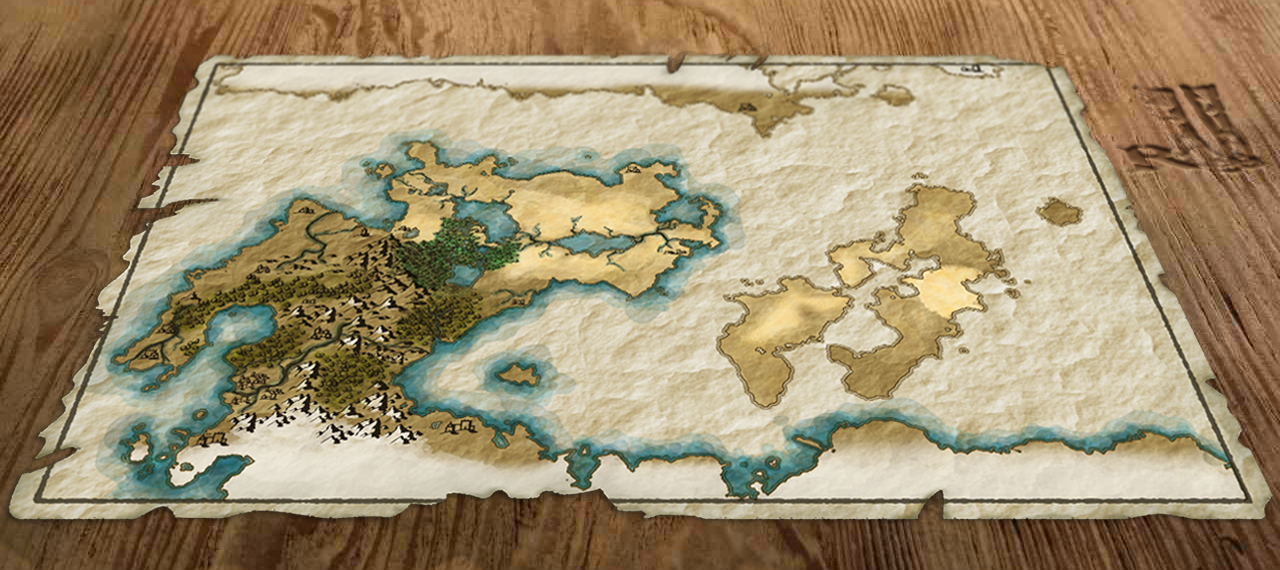
\includegraphics[width=0.7\linewidth]{001.jpg}\vspace{-10pt}
			\nonumber\vspace{-10pt}
		\end{figure}
	\end{itemize}
\end{frame}

\begin{frame}[fragile]{Gain function}
	\begin{itemize}[<+->]
		\item Now we introduce the idea of \textbf{Gain function}:\\
		\begin{equation}
		{\color{blue}Gain_{Bob}} ({\color{blue}\overrightarrow{x}}, {\color{red}\overrightarrow{y}}, {\color{blue}i}) = max\{{\color{blue}B}({\color{blue}\overrightarrow{e_i}}, {\color{red}\overrightarrow{y}})-{\color{blue}B}({\color{blue}\overrightarrow{x}}, {\color{red}\overrightarrow{y}}), 0\} \ \  \ \ \ \ \ \nonumber
		\end{equation}
		\begin{equation}
		{\color{red}Gain_{Alice}} ({\color{blue}\overrightarrow{x}}, {\color{red}\overrightarrow{y}}, {\color{red}j}) = max\{{\color{red}A}({\color{blue}\overrightarrow{x}}, {\color{red}\overrightarrow{e_j}})-{\color{red}A}({\color{blue}\overrightarrow{x}}, {\color{red}\overrightarrow{y}}), 0\} \ \  \ \ \ \ \ \nonumber
		\end{equation}
		\item In other words, the $Gain$ is equal to the increase in payoff for a player if he were to switch to another strategy.
		\item Obviously, the $Gain$ for all players is 0 in \textbf{Nash Equilibrium}.
	\end{itemize}
\end{frame}

\begin{frame}[fragile]{Proof of Nash' Theorem}
	\begin{itemize}[<+->]
		\item Now we define a function as follows:
		 \begin{equation}
		 {\color{blue}f}({\color{blue}\overrightarrow{x}}, {\color{red}\overrightarrow{y}}, {\color{blue}i}) = \frac{{\color{blue}x_i} + {\color{blue}Gain_{Bob}} ({\color{blue}\overrightarrow{x}}, {\color{red}\overrightarrow{y}}, {\color{blue}i})}{1 + \sum_i{\color{blue}Gain_{Bob}} ({\color{blue}\overrightarrow{x}}, {\color{red}\overrightarrow{y}}, {\color{blue}i})}\ \  \ \ \ \ \ \nonumber
		 \end{equation}
		 \begin{equation}
		 {\color{red}g}({\color{blue}\overrightarrow{x}}, {\color{red}\overrightarrow{y}}, {\color{red}j}) = \frac{{\color{red}y_j} + {\color{red}Gain_{Alice}} ({\color{blue}\overrightarrow{x}}, {\color{red}\overrightarrow{y}}, {\color{red}j})}{1 + \sum_j{\color{red}Gain_{Alice}} ({\color{blue}\overrightarrow{x}}, {\color{red}\overrightarrow{y}}, {\color{red}j})}\ \  \ \ \ \ \ \nonumber
		 \end{equation}
		\item In other words, function $f$ and $g$ tries to boost the probability mass that player places on various pure strategies
		depending on the each one's gains in payoff the player would get by switching to these strategies.
	\end{itemize}
\end{frame}

\begin{frame}[fragile]{Proof of Nash' Theorem}
	\begin{itemize}[<+->]
		\item These function is a map from a 2-dimension space to a 2-dimension space.
		\begin{equation}
		(\overrightarrow{x}, \overrightarrow{y}) \overrightarrow{}(\overrightarrow{x'}, \overrightarrow{y'})\ \  \ \ \ \ \  \nonumber
		\end{equation}
	\end{itemize}
\end{frame}

\begin{frame}[fragile]{Proof of Nash' Theorem}
	\begin{itemize}[<+->]
		\item It is easy to see that this function is continuous. So we can use \textbf{Brouwer’s fixed point theorem}, there is at least one fixed point of the function.
		\item For any fixed point 
		\begin{equation}
		{\color{blue}Gain_{Bob}} ({\color{blue}\overrightarrow{x}}, {\color{red}\overrightarrow{y}}, {\color{blue}i}) = 0, \ \ \  \forall i\in [n] \nonumber
		\end{equation}
		\begin{equation}
		{\color{red}Gain_{Alice}} ({\color{blue}\overrightarrow{x}}, {\color{red}\overrightarrow{y}}, {\color{red}j}) = 0, \ \ \  \forall j\in [n]\nonumber
		\end{equation}
		It can be proved by by contradiction.
		\item Then we claim that any fixed point of this function is a \textbf{Nash equilibrium}.
	\end{itemize}
\end{frame}

\begin{frame}[fragile]{The smile of John Nash}
	\begin{figure}[H]
		\centering
		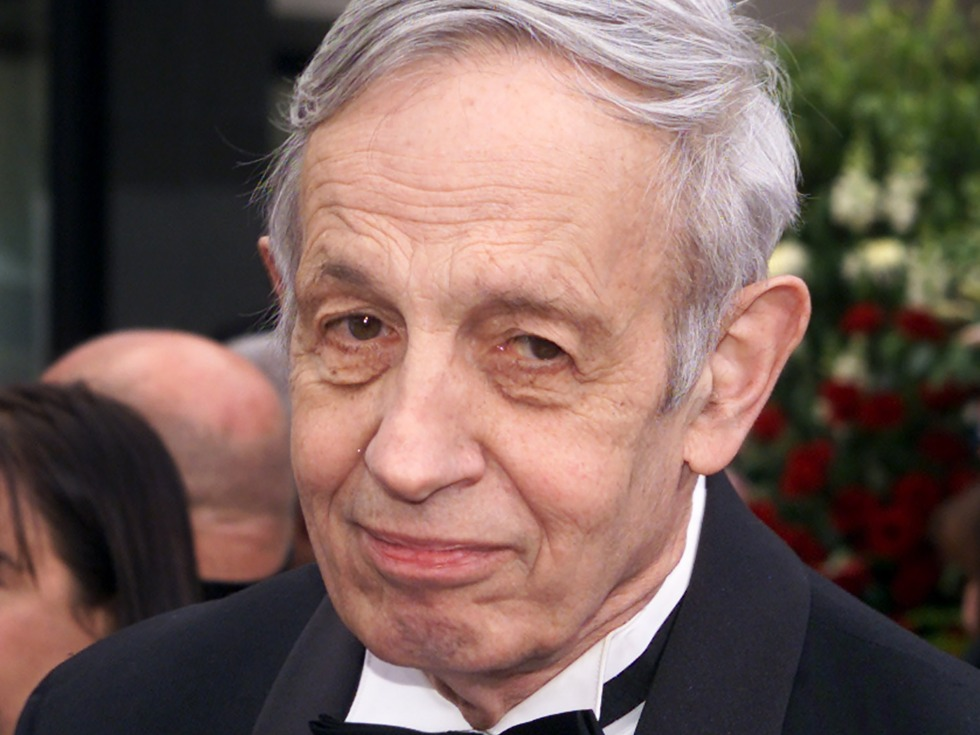
\includegraphics[width=0.7\linewidth]{002.jpeg}\vspace{-10pt}
		\nonumber\vspace{-10pt}
	\end{figure}
\end{frame}


\begin{frame}
\Huge{\centerline{The End}}
\end{frame}


\end{document} 
